% begin module inverse-trig-summary
\begin{frame}[t]
The remaining inverse trigonometric functions aren't used as often:
\[
\begin{array}{llcrcl}
y = \Arccsc x &%
(|x| \geq 1) &%
\alert<0>{\Leftrightarrow}&%
\csc y = x &%
\text{ and } &%
y\in \left(0,\frac{\pi}{2}\right] \cup \left(\pi , \frac{3\pi}{2} \right] \\%
\alert<2>{y = \Arcsec x }&%
\alert<2>{(|x| \geq 1) }&%
\alert<2>{\Leftrightarrow}&%
\alert<2>{\sec y = x }&%
\alert<2>{\text{ and } }&%
\alert<2>{y\in  \left[0,\frac{\pi}{2}\right) \cup \left[\pi , \frac{3\pi}{2}\right) }\\%
y = \Arccot x &%
(|x| \in \mathbb{R}) &%
\alert<0>{\Leftrightarrow}&%
\cot y = x &%
\text{ and } &%
y\in (0,\pi )
\end{array}
\]
\end{frame}
\begin{frame}
We will however make use of $\Arcsec x$: we discuss in detail its domain. 
\[
\begin{array}{llcrcl}
\alert<1>{y = \Arcsec x }&%
\alert<1>{(|x| \geq 1) }&%
\alert<1>{\Leftrightarrow }&%
\alert<1>{\sec y = x }&%
\alert<1>{\text{ and } }&%
\alert<1>{y\in\only<1-6>{\alert<1-6>{\textbf{?}}} \uncover<7->{\alert<7>{ \left[0,\frac{\pi}{2}\right) \cup \left[\pi , \frac{3\pi}{2}\right) }}}
\end{array}
\]

\begin{columns}
\column{0.43\textwidth}
\psset{xunit=0.5cm, yunit=0.5cm}
\begin{pspicture}(-5.2, -5.2)(5.2,5.2) 
\tiny 
\psaxesStandard{-5.15}{-5.15}{5.15}{5.15}

\uncover<1-7>{
\psline[linestyle=dashed](-1.570796327,-5 )(-1.570796327,5)
\psline[linestyle=dashed](1.570796327,-5 )(1.570796327,5)
\psline[linestyle=dashed](4.71238898,-5 )(4.71238898,5)
}
\uncover<10->{
\psline[linestyle=dashed](-5,-1.570796327)(5,-1.570796327)
\psline[linestyle=dashed](-5,1.570796327)(5,1.570796327)
\psline[linestyle=dashed](-5,4.71238898)(5,4.71238898)
}

\psXTickWithLabel{-1.570796327}{$-\frac{\pi}{2}$}
\psXTickWithLabel{1}{$1$}
\psXTick{1.570796327}
\rput[tl](1.6,-0.1){$\frac{\pi}{2}$}
\psXTickWithLabel{3.141592654}{$\pi$}
\psXTick{4.71238898}
\rput[tr](4.65,-0.1){$\frac{3\pi}{2}$}
\psYTickWithLabel{1}{$1$}
\psYTickWithLabel{1.570796327}{$\frac{\pi}{2}$}
\psYTickWithLabel{3.141592654}{$\pi$}
\psYTickWithLabel{4.71238898}{$\frac{3\pi}{2}$}

\uncover<2->{
\rput[l](1.6,4.5){$y=\sec x$}
}
\uncover<9->{
\rput[br](4.9,1.5){$y=\Arcsec x$}
}
\uncover<2-3>{%
%Function formula: 1/\cos{}x 
\psplot[linecolor=\psColorGraph, plotpoints=1000]{-4.511031}{-1.772154}{x 57.29578 mul cos -1 exp }
}%
\uncover<4->{%
%Function formula: 1/\cos{}x 
\psplot[linecolor=gray!10, plotpoints=1000]{-4.511031}{-1.772154}{x 57.29578 mul cos -1 exp }
}%
\uncover<2-3>{%
%Function formula: 1/\cos{}x 
\psplot[linecolor=\psColorGraph, plotpoints=1000]{-1.369438}{0}{x 57.29578 mul cos -1 exp }
}%uncover
\uncover<4->{%
%Function formula: 1/\cos{}x 
\psplot[linecolor=gray!40, plotpoints=1000]{-1.369438}{0}{x 57.29578 mul cos -1 exp }
\psFullDot{0}{1}
}%
\uncover<2->{%
%Function formula: 1/\cos{}x 
\psplot[linecolor=\psColorGraph, plotpoints=1000]{0}{1.369438}{x 57.29578 mul cos -1 exp }
}%
\uncover<2-4,6>{
%Function formula: 1/\cos{}x 
\psplot[linecolor=\psColorGraph, plotpoints=1000]{1.772154}{3.141592654}{x 57.29578 mul cos -1 exp }
}%
\uncover<5,7->{
%Function formula: 1/\cos{}x 
\psplot[linecolor=gray!40, plotpoints=1000]{1.772154}{3.141592654}{x 57.29578 mul cos -1 exp }
\psFullDot{3.141592654}{-1}
}%
\uncover<2-3,5,7->{
%Function formula: 1/\cos{}x 
\psplot[linecolor=\psColorGraph, plotpoints=1000]{3.141592654}{4.511031}{x 57.29578 mul cos -1 exp }
}%uncover
\uncover<4,6>{
%Function formula: 1/\cos{}x 
\psplot[linecolor=gray!40, plotpoints=1000]{3.141592654}{4.511031}{x 57.29578 mul cos -1 exp }
\psFullDot{3.141592654}{-1}
}%uncover
\uncover<8->{%
\psline[linestyle=dashed, linecolor=\psColorTangent](-4.9,-4.9)(4.9,4.9)
}
\uncover<9->{
%Function formula: - \arccos{}(x^{-1})+2 \pi 
\psplot[linecolor=\psColorGraph, plotpoints=1000]{-5}{-1.00001}{ 3.141592654 2 mul x -1 exp ACOS -1 mul add }
%Function formula: \arccos{}(x^{-1}) 
\psplot[linecolor=gray!40, plotpoints=1000]{-5}{-1.00001}{x -1 exp ACOS }
%Function formula: \arccos{}(x^{-1}) 
\psplot[linecolor=\psColorGraph, plotpoints=1000]{1.00001}{5}{x -1 exp ACOS }
%Function formula: -\arccos{}(x^{-1}) 
\psplot[linecolor=gray!40, plotpoints=1000]{1.00001}{5}{x -1 exp ACOS -1 mul}
}
\end{pspicture} 
%\ \only<handout:0| -1>{%
%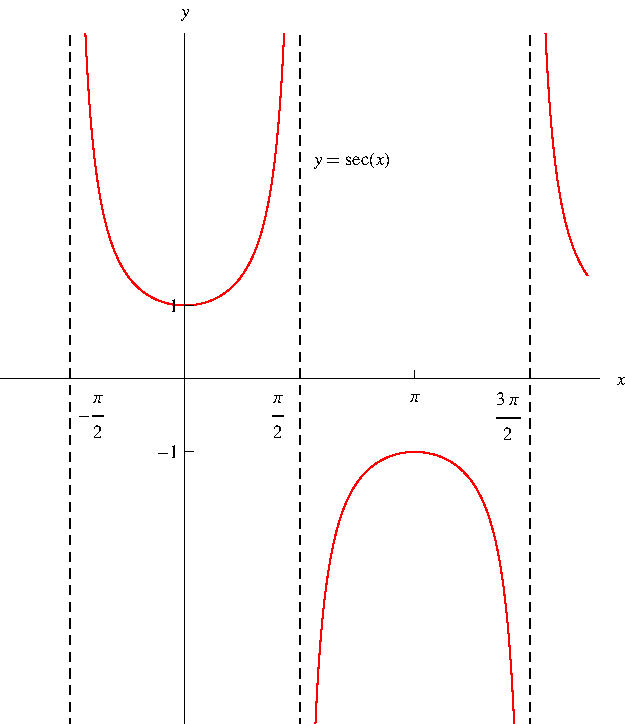
\includegraphics[width=5cm]{inverse-trig/pictures/07-06-seca.pdf}%
%}%
%\only<2->{%
%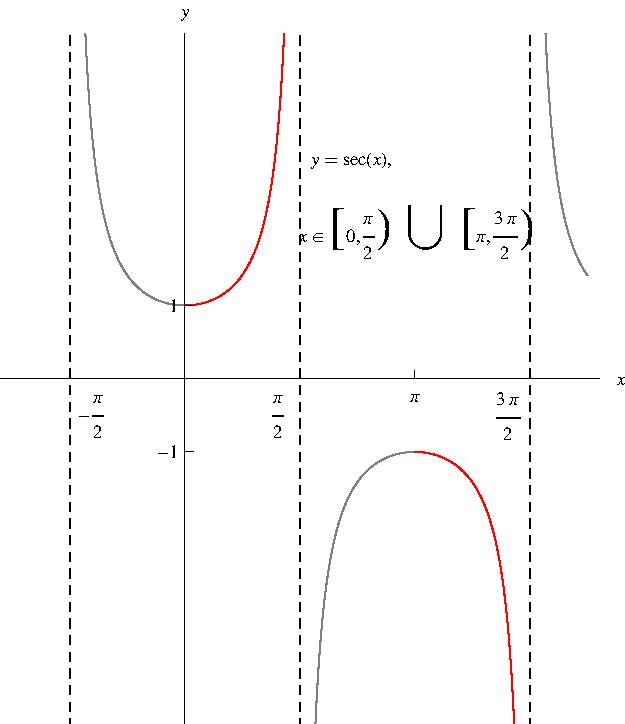
\includegraphics[width=5cm]{inverse-trig/pictures/07-06-secb.pdf}%
%}%
\column{0.57\textwidth}
\begin{itemize} 
\item<2-> \noindent Plot $\sec x$. 
\item<3-> Restrict domain to make one-to-one: Two common choices: \alert<4>{$x\in \left[0, \frac{\pi}{2}\right)\cup\left(\frac{\pi}{2}, \pi \right] $} and \alert<5>{$x\in \left[0, \frac{\pi}{2} \right) \cup \left[\pi,\frac{3\pi}{2} \right) $}. 

\item<6-> $x\in \left[0, \frac{\pi}{2}\right)\cup\left(\frac{\pi}{2}, \pi \right] $ is good because the domain is easiest to remember: an interval without a point. \textbf{NOT our choice.}

\item<7,8,9,10-> $x\in \left[0, \frac{\pi}{2} \right) \cup \left[\pi,\frac{3\pi}{2} \right) $ is  good because $\tan x$ is positive on both intervals, resulting in easier differentiation and integration formulas. \textbf{Our choice.} 

\end{itemize}
\end{columns}

\end{frame}

\begin{frame}
Table of derivatives of inverse trigonometric functions: 
\begin{align*}
\frac{\diff}{\diff x} (\Arcsin x) & = %
\frac{1}{\sqrt{1-x^2}} &%
\frac{\diff}{\diff x} (\Arccsc x) & = %
-\frac{1}{x\sqrt{x^2-1}} \\%
\frac{\diff}{\diff x} (\Arccos x) & = %
-\frac{1}{\sqrt{1-x^2}} &%
\frac{\diff}{\diff x} (\Arcsec x) & = %
\frac{1}{x\sqrt{x^2-1}} \\%
\frac{\diff}{\diff x} (\Arctan x) & = %
\frac{1}{1+x^2} &%
\frac{\diff}{\diff x} (\Arccot x) & = %
-\frac{1}{1+x^2} %
\end{align*}
\end{frame}
% end module inverse-trig-summary
